%\documentclass[a4paper,9pt,fleqn,notoc]{diss}
%% \renewcommand{\includegraphics}[1][1]{} 
%\begin{document}


\chapter{Embodied Cognitive Semantics with IRL}
\label{s:irl}
Artificial agents trying to achieve communicative goals in situated interactions
in the real-world need powerful computational systems for conceptualizing 
their environment. In order to provide 
embodied artificial systems with rich semantics reminiscent of human 
language complexity, agents need mechanisms for both conceptualizing complex 
compositional semantic structure\index{semantic structure}, but, also for 
actively reconstructing semantic 
structure in interpretation of ambiguous utterances.
Furthermore, the system must be open-ended and 
allow agents to adjust their semantic inventories in order to reach their goals. 
This chapter presents the computational system called
Incremental Recruitment Language (IRL)\index{Incremental Recruitment Language} 
that allows agents to represent and process complex conceptualizations\index{conceptualization}
of spatial scenes. The work presented here bases itself on substantial previous work. 
Key ideas of the IRL system have been laid out by \cite{steels2000emergence}\index{Steels, L.}, 
with progress reported in \cite{steels2005planning}\index{Steels, L.}\index{Bleys, J.}, \cite{vandenbroeck2008irl}\index{Van den Broeck, W.}, and
recently in \cite{spranger2010irl,spranger2012irl}\index{Loetzsch, M.}\index{Pauw, S.}\index{Spranger, M.}.

\section{Procedural Semantics}
\label{s:grounded-procedural-semantics}
\begin{figure}
\center
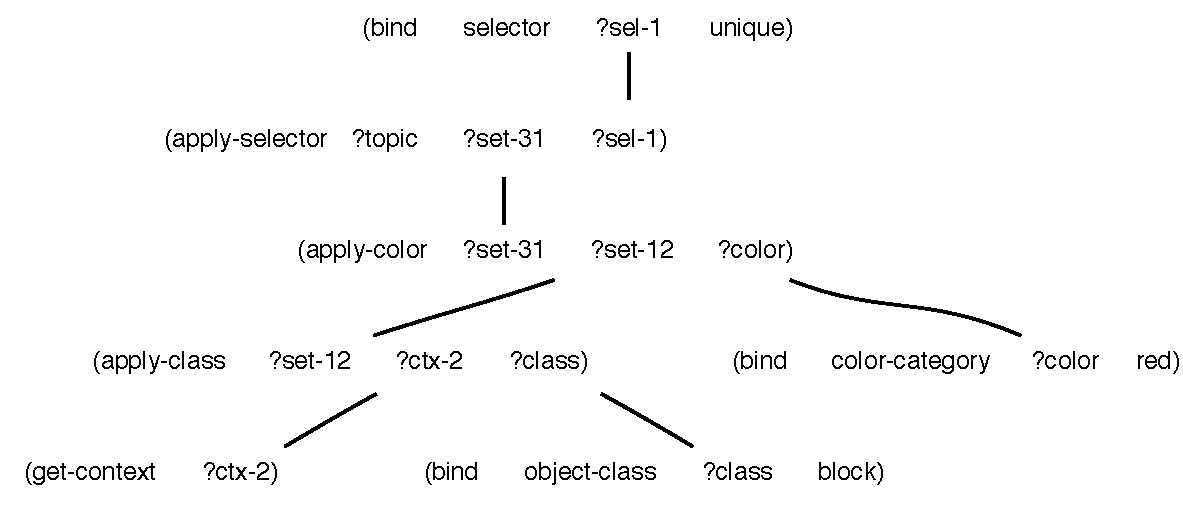
\includegraphics[width=1\columnwidth]{figs/the-red-block-network}
\caption{Semantic structure underlying the utterance ``der rote Block'' (the red block).}
\label{f:the-red-block-network}
\end{figure}

In order for a hearer to interpret an utterance, he has to apply the 
meaning conveyed in the linguistic structure to his perception of 
the context. Consequently, a speaker who 
uses language to achieve a certain communicative goal wants 
the hearer to execute a program \citep{johnson1977procedural}\index{Johnson-Laird, P. N.}, 
i.e. a set of operations that allow the hearer to, for example, discriminate 
an object in the environment or perform an action. Thus we model semantics, 
i.e. what it is a speaker wants the hearer to execute, as a 
program linking operations and data.  Let us start with an example. 
Suppose a speaker utters the phrase ``der rote Block'' (the red block) with the intention 
of making the hearer point to an object. In this case, the phrase 
encodes a program, i.e., set of operations, that are supposed to lead 
the hearer to identify the object in question. Presumably
the hearer of this utterance has to first filter the context for blocks, 
followed by the application of the color category
red, in order to arrive at the set of red blocks, which is used to 
compute the topic consisting of a single entity. A possible program, 
also called \emph{IRL-network}\index{IRL-network|see{semantic structure}}, is shown in Figure \ref{f:the-red-block-network}.
This network explicitly represents the chain of the four operations {\footnotesize\tt get-context},
{\footnotesize\tt apply-class}, {\footnotesize\tt apply-color} and {\footnotesize\tt apply-selector}
by linking their arguments through variables 
(starting with {\footnotesize\tt ?}). The network also 
includes the color category {\footnotesize\tt red}, 
the object class {\footnotesize\tt block} and the selector 
{\footnotesize\tt unique} which are introduced via so called 
\emph{bind statements}, as in 
{\footnotesize\tt (bind color-category ?color red)}. We collectively
refer to concepts, categories etc. as \emph{semantic entities}\index{semantic entity}.

IRL-networks consist of two types of nodes 
\begin{description}
\item[Cognitive operations,] also called \emph{semantic operations},\index{cognitive operation}
are the algorithms used in conceptualization. They encode a particular cognitive 
function such as categorization using a color category,
applying a selector or applying an object class and many more as will be shown
see later in this book for the domain of space. Cognitive operations 
are identified by their name, e.g. {\footnotesize\tt apply-color} and
they have a set of arguments which can be linked to other operations
or semantic entities via variables (starting with {\footnotesize\tt ?}).
\item[Semantic entites] is the general term for referring to prototypes,
concepts and categories that are used by cognitive operations.
Besides such long-term data, semantic entities can also be
discourse representations, the representation of the current context
and data exchanged between cognitive operations. They
are introduced explicitly in the network via {\footnotesize\tt bind}-statements
which are special operations for retrieving the actual data representation
using a pointer or shorthand notation for it. For instance, 
the statement {\footnotesize\tt (bind color-category ?color red)}
encodes the access to the color category {\footnotesize\tt red} which
is a prototype represented using values for different color channels.
\end{description}


\begin{figure}
\center
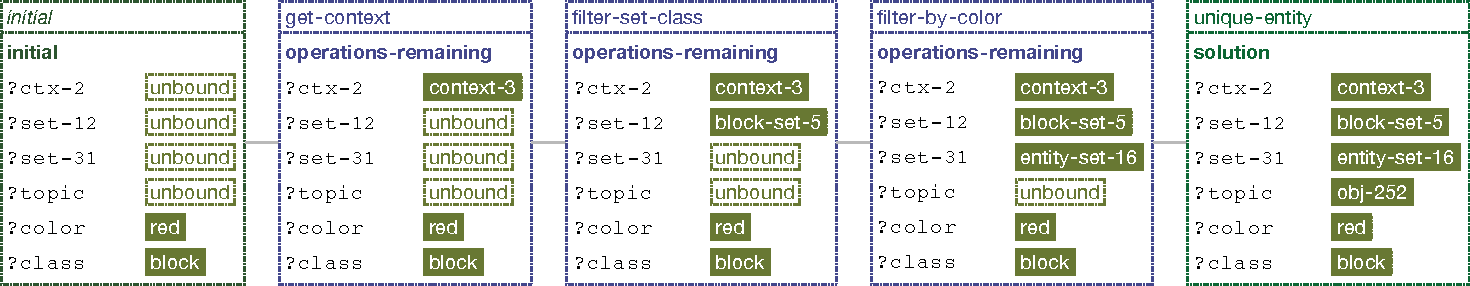
\includegraphics[width=1\columnwidth]{figs/evaluation-tree}
\caption[Evaluation of an IRL-network]{Progressive evaluation 
of the network in Figure \ref{f:the-red-block-network}
on the context shown in Figure \ref{f:scene}.
From left to right, each node represents a step in the evaluation process. From top to bottom, the evaluated operation, the node status, and the current list of bindings of each node are shown. A consistent solution with bindings for all variables is found in the last node, and the value 
{\footnotesize\tt obj-252} is indeed a unique red block (compare \ref{f:scene}).}
\label{f:evaluation-tree}
\end{figure}

\section{Evaluation}\index{cognitive operation!evaluation}
A program such as the one in Figure \ref{f:the-red-block-network} is \emph{evaluated}, 
by a speaker to test the semantic structure with respect to the 
particular communicative goal, or by a hearer in order to interpret an utterance.
Evaluation is a process which cycles over the network and progressively computes values
for variables, a process called \emph{binding}.
When the network in Figure \ref{f:the-red-block-network}
is evaluated the following happens. First {\footnotesize\tt get-context} gets the current 
world model from the perceptual processes that are monitoring the 
environment for events and objects and binds it to the variable 
{\footnotesize\tt ?ctx-2}. This is followed by the evaluation of the {\footnotesize\tt apply-class}
operation which computes a similarity score for how similar every object
in the context is with respect to the object class {\footnotesize\tt block}. 
This yields the set of objects from the context with each object 
scored using the computed similarity. The set is bound to the variable {\footnotesize\tt ?set-12}. 
Because this variable is linked to the operation {\footnotesize\tt apply-color}, 
the set bound to the variable {\footnotesize\tt ?set-12} is further processed using the 
color category {\footnotesize\tt red}. {\footnotesize\tt apply-color} first computes
a similarity score for every object in the input set to the color category 
{\footnotesize\tt red} which is multiplied with the similarity score the object
already has from the application of the class {\footnotesize\tt block}.
This yields a new set of objects with multiplied similarity scores.
The set is bound to the variable {\footnotesize\tt ?set-31}. Lastly, {\footnotesize\tt apply-selector} 
checks the objects in {\footnotesize\tt ?set-31}, finds the object with 
the highest similarity score and binds it to the variable {\footnotesize\tt ?topic}
which is the referent\footnote{Note that the word ``object'' here refers 
to an agent's private representation of 
things he has perceived in the world and only 
indirectly refers to the physical object which is the referent.
} of the phrase ``der rote Block'' (the red block).
Figure \ref{f:evaluation-tree} gives an idea how variables get progressively 
bound when the IRL-network is evaluated.

This is only one example how such a network can be evaluated. 
As has been argued in \cite{steels2000emergence}\index{Steels, L.},
language requires that semantic structure does not encode control flow, but rather 
data flows in all directions and is computed wherever possible.
For this, operations need to be able to function in different directions with
varying input-output parameters
For instance, the operation {\footnotesize\tt apply-class} which has three arguments, 
applies a class such as {\footnotesize\tt block} to an input set, when the 
class is explicitly represented in the network. But, in case
this class is not introduced via a bind statement in the network, the operation
can also provide this information effectively turning this argument
into an output argument. This \emph{multidirectionality}\index{cognitive operation!multidirectionality} of operations 
proves important for dealing with missing items, for instance due to partial parsing 
of an utterance, but it is also needed when constructing semantic structure.


\section{Conceptualization and Interpretation}\index{conceptualization}\index{interpretation}
\begin{figure}
\center
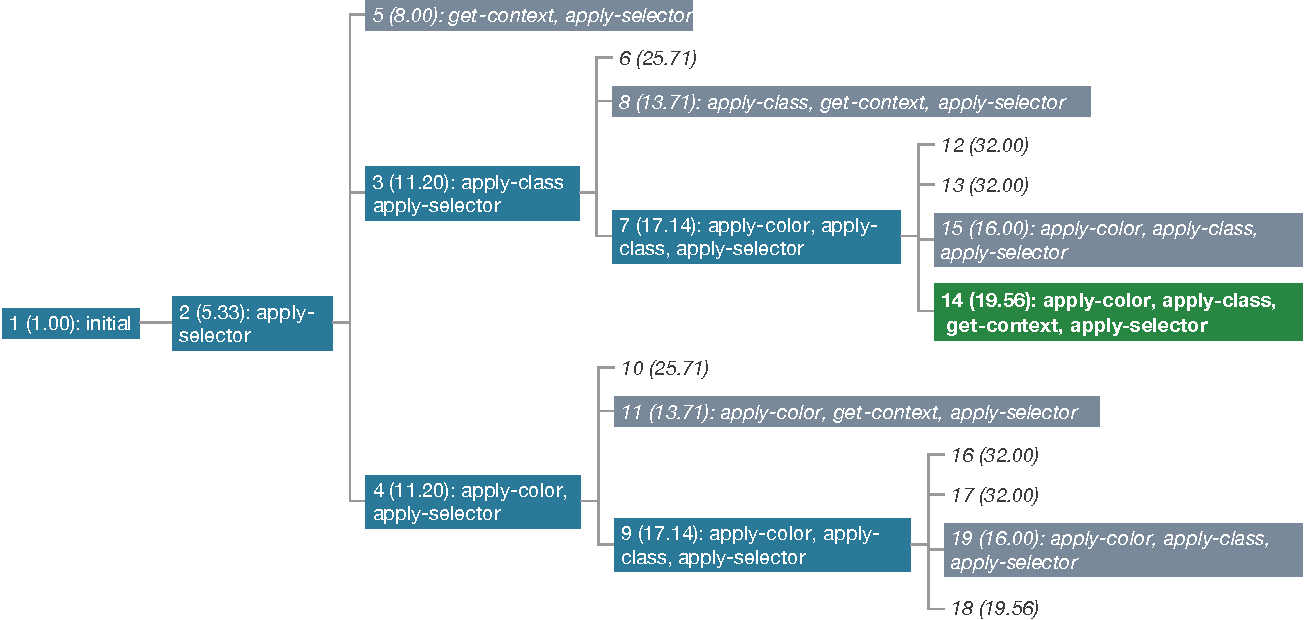
\includegraphics[width=1.0\columnwidth]{figs/composition}
\caption[IRL conceptualization search tree]{The search tree 
for finding the semantic structure seen in 
Figure \ref{f:the-red-block-network}. From left to right, nodes 
represent progressively growing programs combined from 
several chunks, which are each tried out and in some cases 
lead to solutions (green nodes).}
\label{f:the-red-block-search-tree}
\end{figure}

There are two scenarios in which agents autonomously compose semantic
structure like the one just described (Figure \ref{f:the-red-block-network}). 
First, speakers have a particular communicative goal and need to construct 
semantic structure, for instance, for singling out the particular topic the 
speaker wants to draw attention to.
This process is called \emph{conceptualization}. In the second scenario, 
hearers use information parsed from the observed utterance and their 
knowledge about the current context of the interaction to 
actively reconstruct meanings from the potentially partial 
structures parsed by the language system. We call this process 
\emph{interpretation}. Both cases are equally important and
they both conceive the process of building semantic structure as a heuristically
guided search process that explores the space of possible IRL-networks 
driven by the agent's particular communicative goal and the information
available to him.

In conceptualization, in other words while ``planning what to say'' 
\citep{steels2005planning}\index{Steels, L.}\index{Bleys, J.}, a speaker searches for an IRL-network 
that, when executed by the hearer, will reach a particular given 
communicative goal in a particular context.  IRL-networks 
are constructed by assembling basic building
blocks, in particular, cognitive operations packaged into chunks
into more and more complex semantic structures. 
Each assembled structure is immediately tested by evaluating it which assesses
its compatibility with the current communicative goal and the perceived context.
Figure \ref{f:the-red-block-search-tree} shows an example of such a search process 
that has produced the program in Figure \ref{f:the-red-block-network} for discriminating 
the red block in Figure \ref{f:scene}. 
The search process for `good' semantic structure is guided by 
many different heuristics, one being that the structure can be expressed using the
language system available to an agent. Others are more focused on the particular
character of the communicative goal. If the goal is to discriminate an object 
in the environment, then it is beneficial to use more discriminative categories, 
i.e. categories that enlarge the distance between the similarity of the topic and 
the similarity of all other objects in the context. 

Search is also applied when an agent perceiving an utterance  tries to 
interpret it. The semantic structure an agent 
parsed from an utterance is often incomplete and
semantic entities, cognitive operations and links can be
missing in the network. Interpretation is a flexible, active process
by which agents use search to add missing items to the network.
Networks are immediately evaluated to see if they find a referent for 
the parsed utterance. The search process is constrained by the partial 
meaning parsed from the utterance and
the kinds of semantic structures that are appropriate in the current context.
The same scoring mechanisms
as for conceptualization ensures that only structure that is 
discriminating for a particular object (implicitly assuming that the 
speaker constructs structure based on these principles) will be considered 
and the best of all possible results is chosen as the interpretation of an utterance. 

\section{Chunking}\index{chunking}
Search spaces quickly become intractable because the number of 
possibilities for composing semantic structures increases exponentially 
with the number of cognitive operations. A look at language
is helpful here. Grammar can be analyzed as a sophisticated
tool that highly structures human language in order to manage not only
the search space of possible syntactic structure \citep{steels2006dampen}\index{Steels, L.}\index{Wellens, P.} but
perhaps more importantly the vast space of possible conceptual
structures. Parts of meaning that are covered by a particular
part of language can be stored as a \emph{chunk} and 
then used as an basic atomic unit in composition.
Ready-made semantic structure dramatically reduces the search space. If a structure like
the final structure in Figure \ref{f:the-red-block-network} is
constructed from scratch using simple operations, the search tree
would have a search depth of three (essentially one step in depth per
operation). However, every time an operation is added to a program, it
can be linked to the current structure in multiple ways, which leads
to an explosion of nodes on every layer of depth. Hence, the system
soon has to deal with a wide search tree, where every node will be 
executed and tested against the context. Consequently, using chunking 
dramatically increases the performance of the system, even in simple examples.

Chunks have an important role in the study of language because
they package strategies for conceptualizing reality.
Chunks allow to research how cognitive operations
form strategies for conceptualizing reality, how these
strategies can be adapted by agents and how strategies
become conventionalized. For studying conventionalization, 
chunks have scores. This allows to track the success of each strategy with
respect to the communicative goals, e.g. discriminative power
of a strategy, but also with respect to communicative success. 
Strategies for conceptualizing reality are tightly linked to 
language. For instance, one can image that the
chunk in Figure \ref{f:the-red-block-chunk} which 
is extracted from the network in Figure \ref{f:the-red-block-network}
could be the semantics expressed by a determined adjective
noun phrase construction. One important claim is that the structure in language, 
in particular in grammar is tightly connected to the conceptualization
of reality underlying every utterance. So the fact that in English
noun phrases have determiners or, for instance, that in Russian all
verbs are marked for aspects suggests that these languages 
require speakers to conceptualize reality in a certain way and
mark these conceptualizations in language. 



\begin{figure}
\center
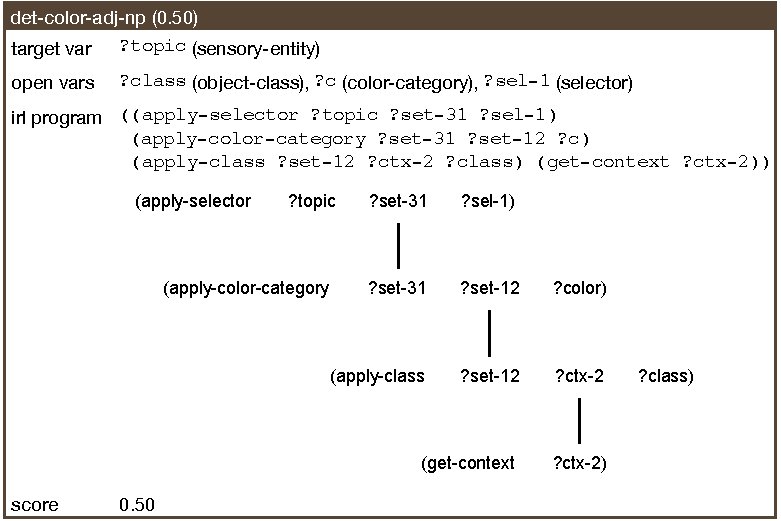
\includegraphics[width=1.0\columnwidth]{figs/det-color-adj-np-chunk}
\caption[Color-adjective noun phrase chunk]{Chunk representing the 
meaning of a determined color-adjective noun phrase. Chunks consist 
of an IRL-network, plus additional information used for processing: 
a target variable and open variables. These variables are typed 
(see brackets for type information)
and they are used in conceptualization and interpretation for combining chunks
to larger structures. The target variable of a chunk can be linked to the open
variable of another chunk. Which selector is used, 
which object class and which color category are is mostly
determined by evaluating the network which yields bindings for
the variables. Since the corresponding variables are open variables
the information can also be provided by other chunks or in interpretation
by the actual lexical items observed in the utterance. Chunks also have a score
which can reflect the degree to which they are conventional 
ways of conceptualizing reality.}
\label{f:the-red-block-chunk}
\end{figure}


\section{Grounding}\index{grounding}
Another important issue is grounding. 
There are now many proposals of how agents can ground lexicons and 
categorical systems in sensorimotor interaction with the environment 
\citep{billard1998grounding,vogt2001bootstrapping,steels2008grounding}\index{Billard, A.}\index{Steels, L.}\index{Dautenhahn, K.}\index{Vogt, P.} and 
IRL is designed to allow such 
insights to be applied straightforwardly. For instance, the 
implementation of the operation for {\footnotesize\texttt{apply-color}} is in part based on 
findings about how basic color categories can be grounded in the sensor 
data streams of digital cameras \citep{steels2005coordinating,bleys2009grounded}\index{Steels, L.}\index{Bleys, J.}\index{Spranger, M.}\index{Belpaeme, T.}\index{Loetzsch, M.}.
Similarly, other grounding mechanisms such as for events 
\citep{siskind2001grounding,steels2003events}\index{Siskind, J. M.}\index{Steels, L.}\index{Baillie, J.-C.} are easily instantiated in IRL operations. 

One of the main claims in this book is that agents co-evolve syntax 
and semantics. Chunks are one way in which agents can
shape strategies for conceptualizing reality. Another
is related to the semantic entities themselves and the fact that the
number of prototypes and categories and their particular 
representation is not fixed. For instance, there is now 
abundant research in the formation of basic color categories 
\citep{steels2005coordinating,belpaeme2007language}\index{Steels, L.}\index{Bleys, J.}\index{Belpaeme, T.}
and how agents can invent, adopt and shape their inventory
of color categories based on the environment they are
facing. These insights into adaptive categories,
but also names and individuals can be incorporated into
IRL which provides mechanisms for the creation and
adaptation of categories in semantic structure.


\section{Discussion}
IRL is a powerful system that for the first time allows 
to study complex semantic phenomena that go beyond
purely lexical studies. IRL is a general system for 
representing the procedural semantics
of utterances. It establishes a link between perception and
language by providing a mechanism for representing the meaning
of utterances, finding and interpreting the meaning of utterances.
Moreover, IRL is designed to allow language processing
to be a flexible, adaptive process which can be extended
by new cognitive operations, new chunks, and new categories 
at any moment. Moreover, IRL provides mechanisms for
tracking the success of semantic material such as 
chunks and categories. 


The oldest and in some sense most similar system 
to what I have presented here is Winograd's SHRDLU 
\citep{haddock1989computational,winograd1971procedures}\index{Haddock, N. J.}\index{Winograd, T.}, However, SHRDLU misses the key aspects of grounding, active interpretation and conceptualization 
as a search process. Other work such as \cite{bailey1997modeling}\index{Bailey, D.}\index{Narayanan, S.}\index{Feldman, J.}
and \cite{siskind2001grounding}\index{Siskind, J. M.} 
focus mostly on lexical meaning. Some approaches
have taken more general approaches e.g. to event structure \citep{narayanan1999moving}\index{Narayanan, S.} 
but stay mostly tied with that particular domain. One of the few approaches talking about 
objects and events in the same framework is \cite{roy2005semiotic}\index{Roy, D.}, which is comparable 
to ours, but so far has been a theoretical proposal only.


%\bibliographystyle{diss}
%\bibliography{papers,space} 
%\end{document}


